%% artigo-exemplo.tex

\documentclass[a4paper]{IEEEtran}
\usepackage[utf8]{inputenc}
%\usepackage{latin}
\usepackage[pdftex]{graphicx}  
\usepackage{epstopdf}
\usepackage{siunitx}




%\usepackage[pdftex]{graphicx}  

\sisetup{
	load-configurations=binary,
	detect-all,
	group-digits=false,
	output-decimal-marker={,},
	per-mode=symbol,
	per-symbol=/,
	binary-units = true
}
\markboth{Provas de Dissertação do MIEEC --- Junho de 2017}{}
\usepackage[portuges]{babel}

%\ifCLASSINFOpdf
%  \usepackage[pdftex]{graphicx}  
%\else
%  \usepackage[dvips]{graphicx}
%\fi

\renewcommand{\footnoterule}{\noindent\rule{0.5\columnwidth}{0.5pt}\vspace*{3pt}}
\graphicspath{{figures/}}
\begin{document}

% Título (usar \\ para quebra de linha)
\title{Implementação em FPGA de um conversor HDMI para transmissão em série de alta velocidade}


% author names and affiliations
% use a multiple column layout for up to three different
% affiliations
\author{\IEEEauthorblockN{Marisa Oliveira$^*$}%
\thanks{$^*$ee12180@fe.up.pt}
\IEEEauthorblockN{João Paulo de Castro Canas Ferreira$^\dag$}%
\thanks{$^\dag$jcf@fe.up.pt}
\IEEEauthorblockN{Henrique Manuel de Castro Faria Salgado$^\ddag$}%
\thanks{$^\ddag$hsalgado@fe.up.pt}
}
% make the title area
\maketitle

% \markboth{Uma parte}{Outra parte}

\begin{abstract}
A sociedade atual depende cada vez mais dos serviços de comunicações, exigindo melhores ligações e mais rápidas, prevendo-se num futuro próximo a necessidade de ligações na ordem das centenas de \SI{}{\giga\bit\per\second}. O projeto \textit{iBrow} que está a ser desenvolvido por vários parceiros, incluindo o INES-TEC, vem propor uma nova exploração do espetro de frequências permitindo assim comunicações de alta velocidade. Este projeto passa por propor uma metodologia que permite a manufaturação de transcetores de baixo custo capazes de atingir grandes débitos de transmissão. A interface HDMI é cada vez mais usada em todos os tipos de ambientes: tanto empresariais como domésticos. Por esse motivo acaba por ser uma boa interface para testar os transcetores que estão a ser desenvolvidos. E por isso, nesta dissertação, é proposto um projeto cuja motivação passa por testar os mesmos. 

O trabalho realizado consiste no desenvolvimento e implementação de  uma arquitetura em FPGA capaz de suportar sinais provenientes de uma fonte HDMI, serializá-los e ainda enviá-los a alta velocidade. A arquitetura suporta ainda o processo inverso, isto é, recebe os dados em série em alta velocidade e envia-os de seguida para um dispositivo HDMI de destino. Para cumprir os requisitos propostos o projeto é dividido em duas partes.
\end{abstract}

%\begin{IEEEkeywords}
%Três ou quarto palavras-chave em ordem alfabética.
%\end{IEEEkeywords}

\section{Introdução}

\IEEEPARstart{E}{ste} documento contempla o trabalho desenvolvido na Dissertação do Mestrado Integrado em Engenharia Eletrotécnica pela Faculdade de Engenharia da Universidade do Porto. 
O objetivo desta passa por transmitir dados HDMI em série a alta velocidade. Para tal, é utilizada uma FPGA que, segundo \cite{R008}, permite desenvolver e implementar uma arquitetura adequada e são também usadas duas placas HDMI que permitem a conversão dos dados HDMI para dados em paralelo. A figura \ref{fig:1} apresenta o diagrama geral do objetivo proposto nesta dissertação.

\begin{figure}[h!]
	\centering
	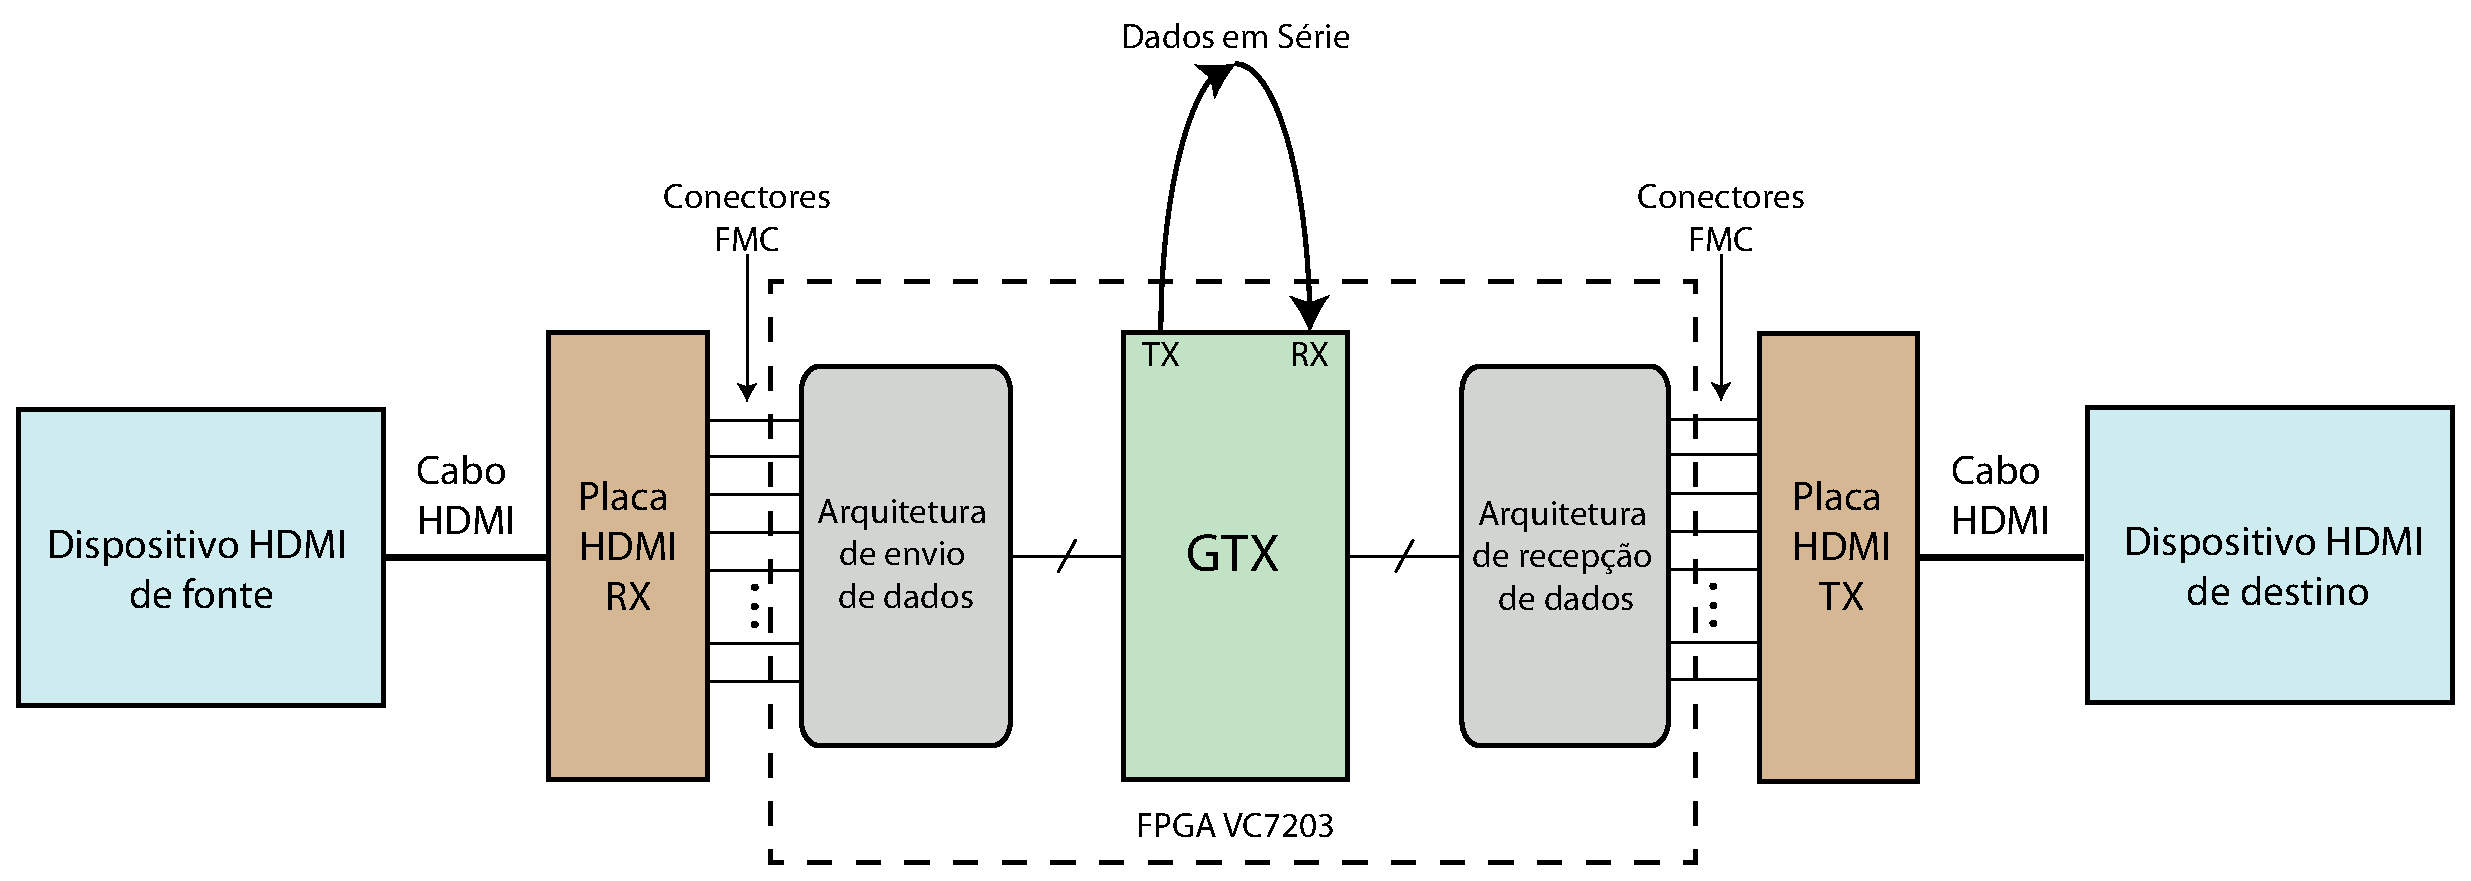
\includegraphics[width=\linewidth]{diagrama_inicial}
	\caption{Diagrama geral do objetivo proposto}
	\label{fig:1}
\end{figure}

\section{Concepção e Desenvolvimento}
Nesta secção são apresentas as duas principais fases do projeto e o trabalho desenvolvido para alcançar o objetivo em cada uma delas.

\subsection{Transmissão de dados HDMI}
A primeira fase do projeto consiste em transmitir dados HDMI entre dois dispositivos de uma forma direta. Foram desenvolvidas diversas arquiteturas no sentido de explorar as diferentes configurações das placas HDMI disponíveis para a concepção do trabalho.
\\
\subsubsection{Transmissão de barra de cores gerada na FPGA para dispositivo HDMI final}
Esta arquitetura utiliza a placa HDMI transmissora configurada por omissão, tal como referenciado em \cite{R009}. Foi desenvolvido um módulo na FPGA que gera uma barra de cores em \textit{FULL HD} com uma taxa de atualização vertical de \SI{60}{\hertz}, que posteriormente envia os dados referentes à mesma para a placa transmissora. 
\\
\subsubsection{Transmissão de imagem entre dispositivos HDMI}
Esta arquitetura utiliza as placas HDMI transmissora e recetora configuradas por omissão, e permite a transmissão de imagem entre dois dispositivos HDMI. Os dados são recebidos pela placa recetora, e diretamente enviados para a placa HDMI transmissora.
\\
\subsubsection{Transmissão de imagem e som entre dispositivos HDMI}
Esta arquitetura, utiliza ambas as placas HDMI configuradas para suporte de um canal e áudio, tal como mencionado em \cite{R014}. Esta mesma assemelha-se à arquitetura desenvolvida no ponto anterior, com a vantagem de ser capaz de transmitir também dados de som.

\subsection{Transmissão de dados HDMI em série}
A segunda fase do projeto consiste no desenvolvimento de uma arquitetura que, com o auxílio dos transcetores disponíveis na FPGA utilizada (cujo manual é referenciado em \cite{R011}), seja capaz de transmitir dados HDMI em série de alta velocidade entre dispositivos.
\\
\subsubsection{Transmissão em série de barra de cores gerada na FPGA para dispositivo HDMI final}
Esta arquitetura utiliza a placa HDMI transmissora configurado por omissão e transmite a imagem resultante do bloco gerador de barra de cores, anteriormente mencionado. Os dados referentes à imagem são transmitidos em tramas de 40 bits a uma cadência de \SI{148.5}{\mega\hertz} de acordo com um determinado formato. Os dados são transmitidos através dos transcetores da FPGA e posteriomente recuperados para o seu envio para a placa HDMI transmissora.
\\
\subsubsection{Transmissão em série de imagem entre dispositivos HDMI}
Esta arquitura utiliza ambas as placas HDMI configuradas por omissão, permitindo que os dados recebidos pela placa recetora sejam enviados em série pelos transcetores da FPGA. Estes dados são também enviados a uma cadência de \SI{148.5}{\mega\hertz} em tramas de 40 bits. Posteriormente são recuperados e enviados para a placa HDMI transmissora.

\section{Principais Resultados Obtidos}
Nesta secção são apresentados os resultados obtidos em cada uma das fases do projeto desenvolvido.
\subsection{Transmissão de dados HDMI}
Relativamente ao trabalho desenvolvido na primeira parte do projeto, obteve-se os resultados esperados atigindo-se assim os objetivos propostos: transmissão direta entre dois dispositivos HDMI explorando as diferentes configurações das placas utilizadas.

\subsection{Transmissão de dados HDMI em série}
Os resultados obtidos relativamente à segunda parte do projeto foram os esperados: foi possível obter uma ligação em série com uma taxa de débito de \SI{5.94}{\giga\bit\per\second} e ainda recuperar devidamente o sinal transmitido. Contudo, surgiu um problema na transmissão de imagem em série entre dispositivos HDMI. Após várias análises, concluiu-se que tal problema não se deve à transmissão em série, mas a um problema de sincronismo ainda antes do envio das tramas para os transcetores. Este pode ser resolvido através da criação de um protocolo de comunicação mais robusto.

\section{Conclusões}

Neste capítulo são apresentadas as considerações finais sobre o projeto desenvolvido tendo em conta a qualidade dos resultados obtidos. São ainda apresentadas algumas propostas de trabalho futuro que visa melhorar o já desenvolvido.

\subsection{Qualidade dos resultados obtidos}

O objetivo principal da primeira parte do projeto é explorar as diferentes configurações das placas HDMI e conseguir obter resultados que venham a ser aplicados na segunda fase do mesmo. Como tal, os resultados obtidos nesta fase foram ao encontro dos objetivos definidos. Foram desenvolvidas e validadas diversas arquiteturas para diferentes configurações das placas HDMI que devido às suas características vieram facilitar a segunda fase do projeto.

Relativamente à transmissão de dados em série, também se conclui que o seu desenvolvimento veio ao encontro dos objetivos definidos para essa mesma fase. A transmissão em série de dados foi obtida com sucesso através do desenvolvimento de uma arquitetura que, em conjunto com o módulo GTX, é capaz de enviar dados e recebê-los corretamente.

Numa perspectiva geral do projeto, os objetivos foram cumpridos: a transmissão em série de dados entre dois dispositivos HDMI foi conseguida, ainda que possa vir a ser melhorada. 

\subsection{Trabalho futuro}

Todo o trabalho realizado teve como motivação a sua inclusão no projeto \textit{iBrow} no sentido de testar os transcetores desenvolvidos pelo mesmo. Consequentemente, para que tal inclusão seja realizada é necessário fazer algumas melhorias do trabalho desenvolvido, que passam de seguida a ser enumeradas:
\begin{itemize}
	\item \textbf{Protocolo de comunicação mais robusto}: Como já mencionado, neste projeto, optou-se por abordar a serialização de uma forma direta sem criar um protocolo de comunicação robusto. Assim sendo, o recurso a este procedimento vem melhorar o processo de transmissão de dados em série colmatando algumas falhas.
	
	\item \textbf{Implementação de códigos detetores de erros:} Com a inserção do sinal em canais ruidosos é expectável que os sinais sejam alterados. O recurso à implementação de códigos detetores de erros vai permitir que tais alterações dos dados sejam detetadas evitando assim que dados errados sejam transmitidos para o final da cadeia de transmissão.
\end{itemize}

Outros aspectos que podem ser explorados, como trabalho futuro, é a transmissão dos dados de som em série, visto que já foi possível obter essa mesma transmissão de uma forma direta e a utilização da interface DRP do GTX para que haja suporte de diferentes resoluções de imagem.

%\subsection{Equações}
%
%Se usar o Word, procure usar o editor de equações Microsoft Equation
%Editor. As equações devem ser numeradas consecutivamente com o número
%entre parênteses na margem direita, como em (\ref{eq:1}).
%
%\begin{equation}
%  \label{eq:1}  
%  \alpha = \int_0^\pi F(r,\sigma) \cdot d\sigma
%\end{equation}


%\subsection{Figuras}
%
%Deve ser inserida uma (e apenas uma) figura no artigo -- aquela que se
%considere ser a mais representativa do trabalho realizado. Deve ser de
%boa qualidade, a cores ou a preto e branco, num formato que permita a
%conversão para pdf do artigo.
%
%%\begin{figure}[ht]
%%  \centering
%%  \includegraphics[width=.8\linewidth]{tux}
%%  \caption{Incluir apenas uma figura no artigo.}
%%  \label{fig:1}
%%\end{figure}

%\subsection{Tabela}
%
%Pode ser inserida apenas uma tabela no artigo. 
%
%\begin{table}[h]
%\caption{Exemplo de tabela}
%
%\begin{tabular}{|c|ccc|r|}
%  \hline
%$k$ &  $x_1^k$    &   $x_2^k$  & $x_3^k$   & remarks  \\
%        \hline
%0   & -0.3 & 0.6 & 0.7  &  \\
%1   & 0.47102965 & 0.04883157 & -0.53345964  & *\\
%2   & 0.49988691 & 0.00228830 & -0.52246185 & $s_3$ \\
%3   & 0.49999976 & 0.00005380 & -0.52365600  & \\
%4   & 0.5 & 0.00000307 & -0.52359743  & $\epsilon < 10^{-5}$ \\
%7   & 0.5 & 0 & -0.52359878  & $\epsilon < \xi $ \\
%        \hline
%\end{tabular}
%\end{table}





\bibliographystyle{IEEEtran}
\bibliography{myrefs}

\end{document}


